% =============================================================================
% paper_marco2a/main.tex
%
% When Sparsity Stops Mattering:
% k-WTA Effect Collapse Under Extreme Domain Shift
% Author: Luis Roberto Pinho da Silva Junior (Independent research)
%
% Workshop submission target: a definir (NeurIPS Bio-Plausible Learning /
% ICLR workshop / LinkedIn). Decisão admin em #66.
%
% Status: LaTeX consolidado sessão #63 (todas as 6 seções + abstract + 3 figuras).
%
% Compilação local (se pdflatex + bibtex disponíveis):
%   pdflatex main.tex
%   bibtex main
%   pdflatex main.tex
%   pdflatex main.tex
% Sem toolchain local: compilar via Overleaf (upload main.tex + refs.bib + figs/).
%
% Template: article + minimal style. Trocar pelo style file oficial do workshop
% (ex: \usepackage[final]{neurips_2024}) no momento da submissão.
% =============================================================================

\documentclass[11pt]{article}
\usepackage[margin=1in]{geometry}
\usepackage[utf8]{inputenc}
\usepackage{amsmath,amssymb,amsthm}
\usepackage{graphicx}
\usepackage{booktabs}
\usepackage{hyperref}
\usepackage{xcolor}
\usepackage{authblk}
\usepackage[round]{natbib}
\bibliographystyle{plainnat}

% Hyperlinks discretos
\hypersetup{
  colorlinks=true,
  citecolor=blue,
  linkcolor=black,
  urlcolor=blue
}

% --- Title and author ---
\title{When Sparsity Stops Mattering:\\k-WTA Effect Collapse Under Extreme Domain Shift}
\author[1]{Luis Roberto Pinho da Silva Junior}
\affil[1]{Independent research \\ \url{https://github.com/luisroberto0/project-hebb}}
\date{2026}

% =============================================================================
\begin{document}
\maketitle

% =============================================================================
\begin{abstract}
The k-winner-take-all (k-WTA) operation imposes sparsity on learned representations and has been shown to preserve few-shot accuracy in-domain: on Omniglot, a Prototypical Network tolerates 75\% embedding sparsity at a cost of only 1.45 percentage points. We ask whether this tolerance survives cross-domain transfer. Taking CNN-4 ProtoNet encoders trained on Omniglot at four sparsity levels ($k \in \{8,16,32,64\}$), we freeze their weights and evaluate on CUB-200-2011, an intentionally adversarial transfer from binary character strokes to natural bird textures. Across five seeds and 1000 episodes per condition, the in-domain sparsity-accuracy spread of 3.78 p.p.\ collapses to 0.52 p.p.\ cross-domain, with fully overlapping confidence intervals. Source-trained encoders are statistically indistinguishable from random-weight controls, and both are outperformed by a representation-free Pixel kNN baseline. A bottleneck decomposition attributes the recoverable gap to target-domain training (+12.22 p.p.) and input resolution (+15.53 p.p.), not sparsity. Under extreme domain shift, bio-inspired sparsity is neither beneficial nor harmful---it is invisible.
\end{abstract}

% =============================================================================
\section{Introduction}
\label{sec:intro}

Sparse coding is a hallmark of cortical computation: only a small fraction of neurons respond actively to each input, and this sparsity is functionally relevant for energy efficiency and representation separation~\citep{olshausen1996emergence,ahmad2019dense}. In mainstream deep learning, however, learned representations remain predominantly dense---post-ReLU activations typically have 30--50\% density, and no architectural constraint enforces additional sparsity. Recent work has begun to characterize when sparsity-inspired mechanisms are compatible with modern methods. \citet{pinho2026kwta} showed that explicit k-WTA sparse coding applied to the embedding of a Prototypical Network~\citep{snell2017prototypical} preserves few-shot accuracy on Omniglot~\citep{lake2015human}: 75\% of activations zeroed costs only 1.45 p.p.\ (93.10\% vs.\ 94.55\% for the full ProtoNet baseline), and even 87.5\% sparsity retains 90.77\%. That result establishes a positive in-domain claim about k-WTA tolerance.

A natural next question follows immediately: \emph{does the effect persist cross-domain?} Few-shot learning research has increasingly emphasized cross-domain robustness~\citep{triantafillou2020meta,tseng2020cross,chen2019closer}, motivated by the observation that meta-learning methods often degrade sharply when source and target domains differ~\citep{phoo2021self}. If sparse coding is a general principle of efficient representation, the expectation is that k-WTA should preserve at least \emph{some} of its in-domain benefit when an Omniglot-trained encoder is applied to a different visual domain. If, conversely, the effect of k-WTA is tied to in-domain regularities, the sparsity-accuracy curve documented on Omniglot should flatten or disappear under domain shift.

This paper presents a controlled empirical study addressing that question. We take the same CNN-4 ProtoNet encoder studied in~\citet{pinho2026kwta}, train it episodically on Omniglot at four sparsity levels ($k = 8, 16, 32, 64$, corresponding to 87.5\%, 75\%, 50\%, and 0\% sparsity over the 64-D embedding), freeze the weights, and evaluate cross-domain on CUB-200-2011~\citep{wah2011caltech}. The Omniglot $\rightarrow$ CUB transfer is intentionally adversarial: binary character strokes against natural RGB textures of bird species, a setting that fits the ``extreme task differences'' regime described by~\citet{phoo2021self}. To distinguish hypotheses about the source of any residual cross-domain signal, we include a Pixel kNN sanity floor (no encoder, raw pixel distances) and a Random encoder + k-WTA control (CNN-4 architecture, untrained Kaiming initialization, k-WTA applied). To establish a baseline for what is achievable with target-domain training, we also retrain ProtoNet directly on the CUB-200 train split at two resolutions: $28 \times 28$ grayscale (architecturally comparable with the source-trained encoders) and $84 \times 84$ RGB (with adaptive pooling preserving the 64-D embedding; this matches resolutions standard in cross-domain few-shot literature).

\textbf{Main empirical findings.} (i) The four sparsity levels tested cross-domain converge tightly within a 0.52 p.p.\ range (k=8: 21.68\%; k=16: 22.09\%; k=32: 22.20\%; k=64 / vanilla: 22.13\%), with all 95\% confidence intervals overlapping. The 3.78 p.p.\ in-domain spread documented in~\citet{pinho2026kwta} \emph{collapses} cross-domain. (ii) An encoder with random untrained weights followed by k-WTA $k=16$ reaches 21.91\%---statistically indistinguishable from the trained encoders, indicating that source-domain training contributes essentially no transferable signal in this setting. (iii) Pixel kNN, with no encoder at all, reaches 22.81\%, with a confidence interval that does not overlap any of the trained encoders, indicating that successive max-poolings in CNN-4 destroy more cross-domain information than they extract. (iv) ProtoNet retrained directly on CUB at $28 \times 28$ grayscale reaches 34.31\%, and at $84 \times 84$ RGB reaches 49.84\%---establishing that target-domain training (+12.22 p.p.\ over source-trained) and adequate input resolution (+15.53 p.p.\ over the 28-pixel grayscale baseline) are the operative bottlenecks, neither of which sparsity addresses.

The contribution of this work is deliberately empirical and characterizational, not methodological:

\begin{enumerate}
    \item We \textbf{quantify} the cross-domain behavior of k-WTA at four sparsity levels with bootstrap 95\% CIs over five seeds and 1000 episodes per seed, using a single source$\to$target pair (Omniglot$\to$CUB-200) chosen for its extreme distance.
    \item We \textbf{document a k-WTA effect collapse}: the in-domain sparsity-accuracy spread of 3.78 p.p.\ is reduced to 0.52 p.p.\ cross-domain, with overlapping CIs.
    \item We \textbf{decompose the cross-domain bottleneck} quantitatively, showing that target-domain training and input resolution each contribute roughly comparable improvements (+12.2 and +15.5 p.p.), while sparsity contributes none.
    \item We \textbf{characterize anti-transfer}: source-trained encoders perform statistically indistinguishably from random-weight controls in this regime.
\end{enumerate}

We do not claim a new method, biological realism, or a breakthrough mechanism. We claim a precise empirical statement: under extreme domain shift between visually unrelated source and target, an effect that mattered in-domain disappears, and bio-inspired sparsity neither helps nor hurts.

% =============================================================================
\section{Background}
\label{sec:background}

\subsection{Cross-Domain Few-Shot Learning}

Few-shot classification has historically been studied in single-domain settings, where the same dataset provides training and evaluation episodes split by class~\citep{lake2015human,vinyals2016matching,snell2017prototypical,finn2017model}. The cross-domain variant---where training and test episodes are drawn from different visual domains---was systematically defined by~\citet{triantafillou2020meta} (Meta-Dataset), which combined 10 sources (ImageNet, Omniglot, Aircraft, CUB-200-2011~\citep{wah2011caltech}, Quick Draw, Fungi, VGG Flower, Traffic Signs, MSCOCO, MNIST) and demonstrated that no single method dominates across domains. \citet{tseng2020cross} introduced feature-wise transformation layers to simulate distribution shift during meta-training, reporting that a vanilla ProtoNet trained on \emph{mini}-ImageNet drops from 49.4\% in-domain accuracy to 38.0\% on CUB-200 in the 5-way 1-shot setting. \citet{chen2019closer} compared baselines and meta-learning methods systematically on \emph{mini}-ImageNet$\to$CUB and showed that simpler baselines (pretrain plus cosine-similarity classifier) often \emph{outperform} sophisticated meta-learning under domain shift. \citet{phoo2021self} pushed further with the BSCD-FSL benchmark, examining ``extreme task differences'' (ImageNet$\to$ChestX, ISIC, EuroSAT, CropDiseases) and proposed STARTUP, which uses unlabeled target-domain self-training to bridge the gap, reporting that without target-domain adaptation ProtoNet baselines fall to the 22--40\% range in 5-way 5-shot accuracy.

The Omniglot$\to$CUB-200 single-source transfer studied here is, to our knowledge, not directly precedented in this literature. Most cross-domain studies use a natural-image source (ImageNet variants) and natural-image targets, with the source domain typically richer than the target. We deliberately invert this: a binary-character source ($28 \times 28$ grayscale strokes) against a natural-texture target (RGB bird photographs at native $\sim 500 \times 500$ resolution, here resized for compatibility). The resulting domain gap is wider than any pair previously characterized, and consequently makes it possible to test whether properties documented in-domain (e.g., k-WTA tolerance) survive at the limit of transferability.

\subsection{k-WTA and Sparse Coding}

The k-winner-take-all (k-WTA) operation is a generalization of classical winner-take-all competition~\citep{maass2000computational}: given a vector of activations, only the $k$ largest values are preserved and the remaining $n-k$ are zeroed. The operation has direct biological motivation: cortical circuits exhibit sparse activity patterns~\citep{olshausen1996emergence}, and lateral inhibition produces approximate winner-take-all dynamics in many neural systems. In machine learning, k-WTA has appeared in Hierarchical Temporal Memory~\citep{ahmad2019dense} and in Modern Hopfield Networks~\citep{ramsauer2021hopfield}, where sparsity supports exponential capacity and pattern separation.

Within Prototypical Networks specifically, \citet{pinho2026kwta} applied k-WTA to the 64-dimensional final embedding of a CNN-4 ProtoNet, varying $k$ across $\{64, 32, 16, 8\}$ (corresponding to 0\%, 50\%, 75\%, 87.5\% sparsity). On Omniglot 5-way 1-shot, the accuracy curve was nearly flat between 0\% and 75\% sparsity (94.55\% at 0\%, 93.35\% at 50\%, 93.10\% at 75\%, a drop of 1.45 p.p.), with a steeper decline at 87.5\% sparsity (90.77\%). A control with random encoder weights and the same k-WTA operation reached 37.60\%, confirming that the in-domain result depends on training under the sparsity constraint, not on the k-WTA structure applied to arbitrary features. The present paper takes those exact source-trained encoders as inputs and asks whether the in-domain effect survives transfer.

\subsection{Datasets: Omniglot and CUB-200-2011}

\textbf{Omniglot}~\citep{lake2015human} contains 1623 hand-drawn characters from 50 alphabets, 20 instances per character, originally provided as $28 \times 28$ binary images suitable for one-shot benchmarks. We use the standard background/evaluation split (30 alphabets / 20 alphabets) for source training. Following~\citet{pinho2026kwta}, we report 5-way 1-shot performance.

\textbf{CUB-200-2011}~\citep{wah2011caltech} contains 11{,}788 photographs of 200 bird species, with 30--60 images per class at native resolution near $500 \times 500$ RGB. The dataset includes bounding boxes, part locations, and 312 attribute labels (we do not use these annotations). The official \texttt{train\_test\_split.txt} provides a per-image binary split that we adopt without modification: 5994 images for the train split and 5794 images for the test split, with all 200 classes appearing in both. For cross-domain evaluation we use only the test split. For the retrained baseline (Section~\ref{subsec:retrained}), we use the train split.

% =============================================================================
\section{Method}
\label{sec:method}

\subsection{Architecture}
\label{subsec:arch}

We use the standard CNN-4 ProtoEncoder of \citet{snell2017prototypical}: four sequential Conv-BN-ReLU-MaxPool blocks with 64 filters and $3 \times 3$ kernels, padding 1. For an Omniglot input $(1, 28, 28)$, four max-poolings of $2 \times 2$ reduce the spatial output to $1 \times 1$, and we flatten into a 64-dimensional embedding $f_\theta(x) \in \mathbb{R}^{64}$. The k-WTA operation is applied to this embedding; classification then proceeds as in standard Prototypical Networks. The architecture is identical to the C3 encoder of \citet{pinho2026kwta}, enabling direct cross-domain transfer of source-trained weights.

\subsection{k-WTA Layer}
\label{subsec:kwta}

The $k$-winner-take-all operation~\citep{maass2000computational} retains the $k$ largest entries of an activation vector and zeros the rest:
\begin{equation}
\text{k-WTA}_k(z)_i = \begin{cases} z_i & \text{if } i \in \arg\text{top-}k(z) \\ 0 & \text{otherwise} \end{cases}
\label{eq:kwta}
\end{equation}
The operation is applied per-example (not over batches), and the gradient flows through the $k$ active channels via standard backpropagation. We apply k-WTA at both training and evaluation time. When $k \geq \dim(z) = 64$, the operation is a no-op and the encoder is equivalent to the vanilla ProtoNet baseline; we use this as the $k=64$ control.

\subsection{Source Training: Omniglot}
\label{subsec:source}

We train each $(k$-WTA configuration, seed$)$ pair episodically on the Omniglot~\citep{lake2015human} background split (964 characters from 30 alphabets). Each episode samples $N=5$ classes, $K=1$ support example, and $Q=5$ query examples. Training uses cross-entropy on query-to-prototype squared Euclidean distances, optimized with Adam~\citep{kingma2015adam} (learning rate $10^{-3}$, no scheduling, no regularization) for 5000 episodes, following the protocol of \citet{pinho2026kwta}. Sparsity sweep covers $k \in \{8, 16, 32, 64\}$.

\subsection{Cross-Domain Protocol}
\label{subsec:xdomain}

Our primary protocol resizes all images, regardless of source, to $28 \times 28$ and converts them to grayscale, preserving the source-trained encoders' input shape $(1, 28, 28)$. The cost of this choice is severe: $500 \times 500$ RGB photographs reduced to $28 \times 28$ grayscale lose nearly all texture and color information that conventionally distinguishes bird species. We report the impact of this resolution choice in Section~\ref{sec:experiments} via a parallel $84 \times 84$ RGB retrained baseline. The visual distance between Omniglot and CUB-200 is large in any reasonable embedding metric, and we treat the pair as an instance of the ``extreme task differences'' regime~\citep{phoo2021self}.

After source training, encoder weights are frozen (\texttt{requires\_grad=False}) and evaluated on the CUB-200 test split (5794 images, 200 classes, official \texttt{train\_test\_split.txt}). Each (encoder, seed) pair runs 1000 episodes 5-way 1-shot 5-query, sampling deterministically from the test split via per-seed random number generators.

\subsection{Sparsity Sweep}
\label{subsec:sweep}

The four-point sweep ($k \in \{8, 16, 32, 64\}$, sparsity $\{87.5\%, 75\%, 50\%, 0\%\}$) requires 20 source-trained checkpoints across 5 seeds. The $k=64$ configuration, being a no-op on a 64-D embedding, has gradient flow identical to the vanilla ProtoNet baseline. We materialize $k=64$ checkpoints by copying the trained ProtoNet baseline state dictionary with key prefix adjustment (the sparse encoder wraps the base encoder under \texttt{self.encoder.}, so each key is renamed accordingly). Sanity verification confirms that $k=64$ cross-domain accuracy reproduces the ProtoNet baseline result exactly.

\subsection{Sanity Floors}
\label{subsec:floors}

Two control conditions probe the source of the residual cross-domain signal. \textbf{Pixel kNN}: nearest-neighbor classification over raw pixels, with each $(1, 28, 28)$ image flattened to $\mathbb{R}^{784}$ and class prototypes computed as per-class pixel means. No encoder, no learning. \textbf{Random encoder + k-WTA}: a $\text{ProtoEncoderSparse}(k=16)$ initialized with PyTorch's default Kaiming-uniform scheme, weights frozen, no training. Different seeds produce different random encoders.

\subsection{Re-trained Baseline}
\label{subsec:retrained}

To upper-bound what is achievable on this benchmark with target-domain training, we retrain ProtoNet directly on the CUB-200 train split (5994 images, 200 classes) at two resolutions. \textbf{$28 \times 28$ grayscale}: identical CNN-4 architecture as the source-trained encoders; same hyperparameters (5000 episodes, Adam $10^{-3}$). \textbf{$84 \times 84$ RGB}: a CNN-4 variant in which the first layer accepts three input channels and a final \texttt{AdaptiveAvgPool2d}((1,1)) collapses the $5 \times 5$ feature map to a 64-D embedding consistent with the source-trained models. We train 5 seeds per resolution.

\subsection{Evaluation}
\label{subsec:eval}

For each condition, we report mean accuracy across 5 seeds with two confidence intervals: the inter-seed mean $\pm$ standard deviation, and a 95\% bootstrap CI computed by resampling the five per-seed means 1000 times with replacement. Per-seed numbers also include 95\% bootstrap CIs over the 1000 episodes.

% =============================================================================
\section{Experiments}
\label{sec:experiments}

\subsection{Setup}
\label{subsec:setup}

All experiments run on a single workstation with an Intel Core i9 CPU and an NVIDIA RTX 4070 Laptop GPU (compute capability 8.9, 8\,GB VRAM), using PyTorch 2.6 with CUDA 12.4. Source training is approximately 70 seconds per (sparsity, seed) checkpoint; the 20 source-trained checkpoints plus 10 retrained-on-CUB checkpoints total roughly 30 minutes of GPU time. Each evaluation run (1000 episodes for one configuration on one seed) takes between 2 and 6 seconds depending on the encoder. CUB images are pre-processed once and cached on disk: 37\,MB for the $28 \times 28$ grayscale tensor and 280\,MB for the $84 \times 84$ RGB tensor.

\subsection{Cross-Domain Results}
\label{subsec:xdomain-results}

Table~\ref{tab:main} reports 5-way 1-shot accuracy on the CUB-200 test split for the eight characterized conditions, with a chance baseline of 20.00\%.

\begin{table}[tbp]
\centering
\small
\caption{Cross-domain 5-way 1-shot accuracy on CUB-200 test split, 5 seeds $\times$ 1000 episodes each. ``Inter-seed std'' is the standard deviation of the five per-seed means. CIs are 95\% bootstrap intervals on the per-seed means. ``Omniglot frozen'' marks encoders whose weights are not updated for CUB.}
\label{tab:main}
\begin{tabular}{lrrrr}
\toprule
Model & Input shape & Mean ACC & Inter-seed std & 95\% CI \\
\midrule
ProtoNet retrained on CUB ($84 \times 84$ RGB)            & $(3, 84, 84)$  & 49.84\% & 0.82\% & [49.38, 50.59] \\
ProtoNet retrained on CUB ($28 \times 28$ gray)           & $(1, 28, 28)$  & 34.31\% & 0.31\% & [34.06, 34.55] \\
Pixel kNN cross-domain                                    & $(1, 28, 28)$ raw & 22.81\% & 0.18\% & [22.69, 22.97] \\
C3 $k=32$ (50\% sparse, Omniglot frozen)                  & $(1, 28, 28)$  & 22.20\% & 0.53\% & [21.77, 22.57] \\
C3 $k=64$ (vanilla, Omniglot frozen)                      & $(1, 28, 28)$  & 22.13\% & 0.30\% & [21.90, 22.36] \\
C3 $k=16$ (75\% sparse, Omniglot frozen)                  & $(1, 28, 28)$  & 22.09\% & 0.32\% & [21.84, 22.34] \\
Random encoder + k-WTA $k=16$                             & $(1, 28, 28)$  & 21.91\% & 0.17\% & [21.76, 22.03] \\
C3 $k=8$ (87.5\% sparse, Omniglot frozen)                 & $(1, 28, 28)$  & 21.68\% & 0.44\% & [21.34, 22.04] \\
\midrule
Chance                                                    & ---            & 20.00\% & ---    & --- \\
\bottomrule
\end{tabular}
\end{table}

The five conditions using the $(1, 28, 28)$ input through some form of CNN-4 forward pass (the four source-trained sparsities plus the random-encoder control) cluster tightly between 21.68\% and 22.20\%, with overlapping 95\% CIs. Pixel kNN, with no encoder at all, reaches 22.81\%, with a CI that does not overlap any of the encoder-based conditions. ProtoNet retrained directly on CUB at the same $28 \times 28$ grayscale resolution reaches 34.31\%, an absolute improvement of $+12.22$ p.p.\ over the $k=16$ source-trained encoder under the same input pipeline. Increasing the input to $84 \times 84$ RGB raises the retrained baseline to 49.84\%, a further $+15.53$ p.p.

\begin{figure}[tbp]
\centering
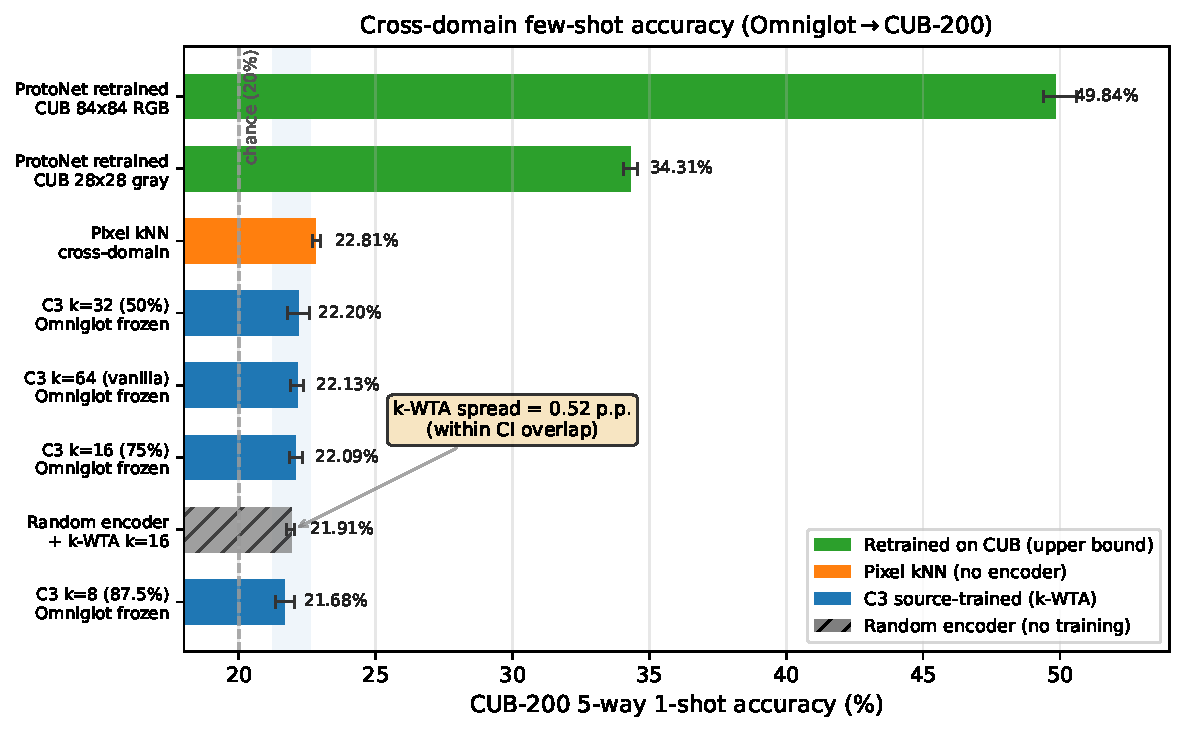
\includegraphics[width=0.92\linewidth]{figs/fig1_crossdomain_bars.pdf}
\caption{Cross-domain 5-way 1-shot accuracy on CUB-200 for all eight conditions of Table~\ref{tab:main}, with the chance line at 20\%. The shaded band marks the five CNN-forward conditions (four source-trained sparsities plus the random encoder), which collapse into a 0.52 p.p.\ spread. Retrained-on-CUB baselines (green) sit well above; Pixel kNN (orange) exceeds every learned encoder.}
\label{fig:crossdomain-bars}
\end{figure}

\subsection{In-Domain vs.\ Cross-Domain Effect}
\label{subsec:effect-collapse}

Table~\ref{tab:effect-collapse} compares the same four sparsity levels on Omniglot (in-domain numbers from \citet{pinho2026kwta}) and on CUB-200 cross-domain. The drop in accuracy from in-domain to cross-domain is approximately 70 p.p.\ across all $k$. Critically, the spread \emph{across} sparsity levels collapses from 3.78 p.p.\ in-domain to 0.52 p.p.\ cross-domain.

\begin{table}[tbp]
\centering
\small
\caption{In-domain (Omniglot) vs.\ cross-domain (CUB-200) 5-way 1-shot accuracy at four sparsity levels. In-domain numbers from \citet{pinho2026kwta}; cross-domain from this work. The bottom row reports the spread (max $-$ min) across the four $k$ values within each domain.}
\label{tab:effect-collapse}
\begin{tabular}{rrrrr}
\toprule
$k$ & Sparsity & Omniglot 5w1s & CUB 5w1s & $\Delta$ in $\to$ cross \\
\midrule
8   & 87.5\%        & 90.77\%         & 21.68\%       & $-69.09$ p.p. \\
16  & 75\%          & 93.10\%         & 22.09\%       & $-71.01$ p.p. \\
32  & 50\%          & 93.35\%         & 22.20\%       & $-71.15$ p.p. \\
64  & 0\% (vanilla) & 94.55\%         & 22.13\%       & $-72.42$ p.p. \\
\midrule
\multicolumn{2}{l}{Spread (max $-$ min)} & 3.78 p.p. & 0.52 p.p. & --- \\
\bottomrule
\end{tabular}
\end{table}

The in-domain spread of 3.78 p.p.\ between $k=8$ and $k=64$ is the empirical signature of k-WTA's effect on ProtoNet documented in \citet{pinho2026kwta}: the cost of imposing 87.5\% sparsity is a measurable accuracy drop of approximately 4 p.p. relative to the unconstrained encoder. Cross-domain, the analogous spread is 0.52 p.p., entirely contained within the overlap of per-condition 95\% confidence intervals. The effect that mattered in-domain becomes statistical noise under transfer.

\begin{figure}[tbp]
\centering
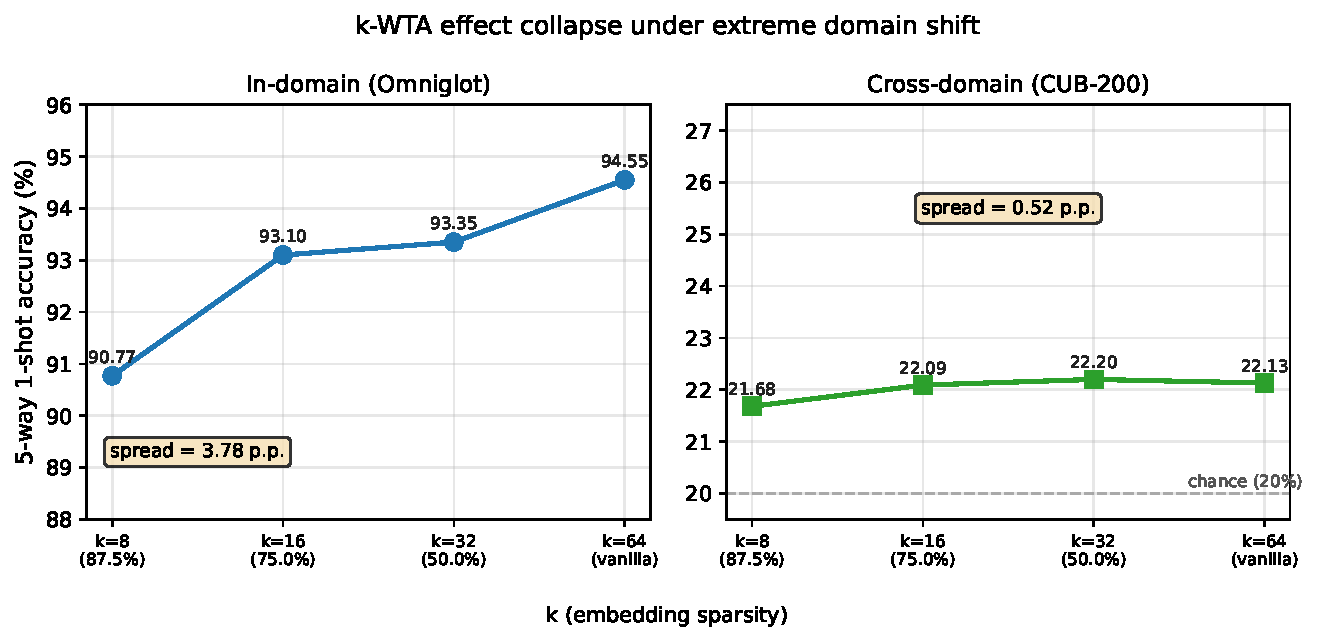
\includegraphics[width=0.95\linewidth]{figs/fig2_effect_collapse.pdf}
\caption{k-WTA effect collapse across sparsity levels. \textbf{Left:} in-domain (Omniglot), accuracy rises with $k$ over a 3.78 p.p.\ spread. \textbf{Right:} cross-domain (CUB-200), the same sweep is flat at $\sim$22\% within a 0.52 p.p.\ spread, just above chance. Both panels share an 8 p.p.\ vertical span.}
\label{fig:effect-collapse}
\end{figure}

\subsection{Bottleneck Decomposition}
\label{subsec:bottleneck}

Successive comparisons isolate where the gap between random-weight and high-performance conditions originates:

\begin{itemize}
    \item \textbf{Random encoder} (21.91\%) $\to$ \textbf{$k=16$ source-trained} (22.09\%): $+0.18$ p.p. The contribution of training on Omniglot, holding the input pipeline fixed, is statistically negligible.
    \item \textbf{$k=16$ source-trained} (22.09\%) $\to$ \textbf{ProtoNet retrained on CUB at $28 \times 28$} (34.31\%): $+12.22$ p.p. With the same input pipeline, switching the training distribution from source to target accounts for over twelve percentage points.
    \item \textbf{Retrained at $28 \times 28$} (34.31\%) $\to$ \textbf{retrained at $84 \times 84$ RGB} (49.84\%): $+15.53$ p.p. With training on the target held fixed, increasing input resolution and adding color contributes another fifteen-and-a-half points.
\end{itemize}

The two large contributors---target-domain training and adequate input fidelity---are of comparable magnitude and roughly additive. Sparsity contributes none.

\begin{figure}[tbp]
\centering
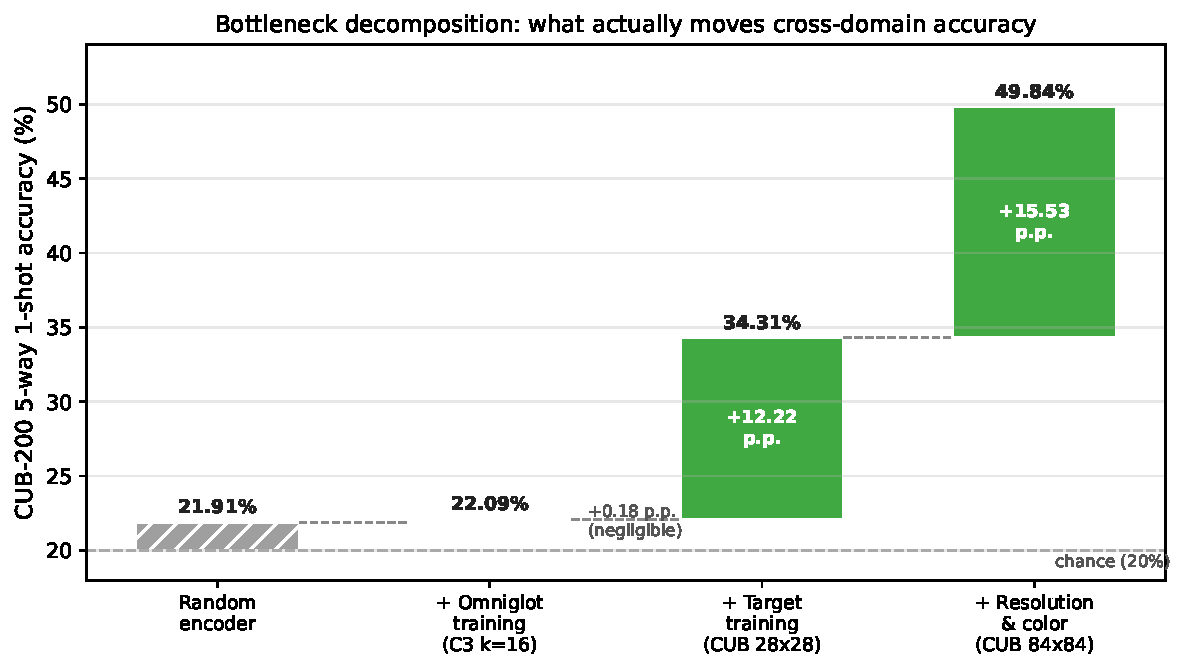
\includegraphics[width=0.92\linewidth]{figs/fig3_bottleneck_waterfall.pdf}
\caption{Bottleneck decomposition as a waterfall. From the random-encoder floor, training on the source (Omniglot, $k=16$) adds a negligible $+0.18$ p.p.; switching training to the target (CUB, $28 \times 28$) adds $+12.22$ p.p.; raising input fidelity to $84 \times 84$ RGB adds $+15.53$ p.p. Sparsity does not appear: the two operative contributors are target training and input fidelity.}
\label{fig:bottleneck}
\end{figure}

\subsection{Anti-Transfer Evidence}
\label{subsec:anti-transfer}

The 0.18 p.p.\ gap between random and source-trained encoders is statistically indistinguishable from zero: the 95\% CI of the random encoder ([21.76, 22.03]) overlaps the CI of the source-trained $k=16$ encoder ([21.84, 22.34]), and the difference is well within seed-to-seed variation. Five thousand episodes of episodic training on Omniglot produce no detectable transferable signal in this regime. We refer to this pattern as \emph{anti-transfer}: an encoder trained on a sufficiently distant source is at best equivalent to an untrained one, and---as the next subsection shows---may underperform a representation that involves no encoder at all. The pattern is consistent with the diagnoses of \citet{phoo2021self}: source-domain training, however thorough, is insufficient under extreme task differences, and self-training on the target domain is required to bridge the gap.

\subsection{Pixel kNN Dominates Encoded Representations}
\label{subsec:pixel-dominates}

Pixel kNN (22.81\%, CI [22.69, 22.97]) outperforms all four source-trained sparsities and the random encoder, with a CI that does not overlap any encoder-based condition (next-highest, $k=32$ at 22.20\%, ends at 22.57\%). To our knowledge, this configuration---an Omniglot single-source CNN-4 transferred to CUB-200 at $28 \times 28$ grayscale---has not been characterized in the cross-domain few-shot literature. The pattern is consistent with \citet{chen2019closer}'s observation that simple baselines often outperform meta-learning under domain shift; the finding here is a stronger version of the same effect, in which a baseline that does not even use a learned representation outperforms multiple variants of one. We discuss likely mechanisms in Section~\ref{sec:discussion}.

% =============================================================================
\section{Discussion}
\label{sec:discussion}

\subsection{Why the k-WTA Effect Collapses Cross-Domain}
\label{subsec:why-collapse}

The in-domain result of \citet{pinho2026kwta} is that constraining a trained 64-D embedding to its $k$ largest coordinates costs little accuracy because the encoder, optimized on Omniglot under that constraint, learns to concentrate class-discriminative information in the surviving coordinates. Cross-domain, two conditions that made the operation meaningful are absent. First, the encoder is never optimized on CUB, so there is no reason for bird-discriminative information to occupy the top-$k$ coordinates of the embedding it produces. Second, and more fundamentally, our results suggest that little such information reaches the embedding at all: Pixel kNN (22.81\%) outperforms every CNN-4 forward pass (21.68--22.20\%) with a non-overlapping confidence interval. The four max-pooling stages that reduce a $28 \times 28$ input to a $1 \times 1$ feature map ($28 \to 14 \to 7 \to 3 \to 1$) appear to discard more cross-domain-relevant signal than they preserve, leaving an embedding that is already near-degenerate before k-WTA is applied. Selecting the top-$k$ of an uninformative vector is itself uninformative, regardless of $k$; the 0.52 p.p.\ spread is what that degeneracy looks like quantitatively.

\subsection{Anti-Transfer Rather Than Neutral Transfer}
\label{subsec:anti-transfer-disc}

The 0.18 p.p.\ gap between source-trained and random encoders (Section~\ref{subsec:anti-transfer}) is the sharper of our findings. Episodic training on Omniglot does not merely fail to help on CUB---it fails to produce any measurable advantage over Kaiming-initialized random weights. We describe this as \emph{anti-transfer} rather than neutral transfer because the trained encoder also does not match the simplest representation-free baseline: Pixel kNN exceeds it. An encoder optimized to separate binary character strokes evidently learns filters whose inductive bias is actively unhelpful for natural textures, to the point that raw pixel distances are preferable to the features it computes. This is consistent with the central premise of STARTUP~\citep{phoo2021self}: under extreme task differences, source-domain training alone is insufficient, and adaptation on the target domain---which our frozen-encoder protocol deliberately forbids---is the operative ingredient. Our setting can be read as an empirical lower bound on what frozen source transfer achieves when the source is maximally distant.

\subsection{Implications for Bio-Inspired Sparsity}
\label{subsec:implications}

Read together with \citet{pinho2026kwta}, these results bound the scope of a bio-inspired sparsity claim rather than refute it. In-domain, k-WTA is \emph{compatible}: 75\% sparsity is essentially free. Cross-domain under extreme shift, k-WTA is \emph{invisible}: it neither recovers nor degrades accuracy because the representation it operates on carries no transferable signal. Sparsity is therefore neither a universal benefit nor a liability; its effect is contingent on the encoder having learned a relevant representation in the first place. For arguments that sparse coding is a general principle of efficient cortical computation, this is a useful boundary condition: the principle's measurable benefit, at least in this prototype-based setting, is inherited from---not independent of---the quality of the underlying features.

\subsection{Relation to Cross-Domain Few-Shot Literature}
\label{subsec:lit-comparison}

Our numbers extend the trend reported across the cross-domain literature to a more extreme point. \citet{tseng2020cross} report a vanilla ProtoNet dropping from 49.4\% in-domain to 38.0\% on \emph{mini}-ImageNet$\to$CUB; our Omniglot$\to$CUB transfer drives the same architecture to 22\%, within 2 p.p.\ of chance. The monotonic relationship between source--target distance and degradation is intuitive, but the magnitude here is notable: the transfer is weak enough that the meta-learned encoder loses to a representation-free baseline. This is a strengthened form of the observation by \citet{chen2019closer} that simple baselines often beat meta-learning under domain shift---in our regime, a baseline that uses no learned representation beats multiple variants of one. We read the Omniglot$\to$CUB pair as a useful stress-test anchor at the far end of the ``extreme task differences'' axis defined by \citet{phoo2021self}.

\subsection{Limitations}
\label{subsec:limitations}

The study is deliberately narrow and its conclusions should not be over-generalized. We use a single source dataset (Omniglot), a single target dataset (CUB-200), and a single backbone (CNN-4); we did not test ResNet or transformer encoders, which have different pooling structure and might preserve more cross-domain signal. Our primary input pipeline is $28 \times 28$ grayscale, chosen for architectural comparability with the source-trained encoders; the $84 \times 84$ RGB result enters only through the retrained baseline. We apply k-WTA only at the final embedding, not at intermediate layers, and we do not test any target-domain adaptation. Each of these is a plausible reason the collapse might be less complete in a different configuration.

\subsection{Future Work}
\label{subsec:future-work}

Three directions follow directly. First, varying source--target distance---e.g.\ \emph{mini}-ImageNet$\to$CUB versus Omniglot$\to$CUB under an identical k-WTA sweep---would test whether the effect collapse is gradual or threshold-like. Second, applying k-WTA at intermediate convolutional layers, rather than only the embedding, would test whether sparsity interacts with cross-domain features before pooling destroys them. Third, integrating target-domain self-training (STARTUP-style)~\citep{phoo2021self} would test whether the anti-transfer pattern reverses once the encoder is allowed to adapt. Extending to multiple targets (Cars, Places, Plantae) would establish whether the collapse generalizes beyond the single Omniglot$\to$CUB pair characterized here.

% =============================================================================
\section{Conclusion}
\label{sec:conclusion}

We characterized the cross-domain behavior of k-winner-take-all sparsity by transferring CNN-4 Prototypical Network encoders trained on Omniglot, at four sparsity levels, to CUB-200-2011, evaluated over five seeds and 1000 episodes each with bootstrap confidence intervals. The in-domain sparsity-accuracy spread of 3.78 p.p.\ reported by \citet{pinho2026kwta} collapses to 0.52 p.p.\ under this extreme domain shift, entirely within the overlap of per-condition confidence intervals. A decomposition of the residual gap shows that target-domain training (+12.22 p.p.) and adequate input resolution (+15.53 p.p.) are the operative bottlenecks, while sparsity contributes none; a source-trained encoder is statistically indistinguishable from a random-weight control, and both are outperformed by a representation-free Pixel kNN baseline.

The practical implication is narrow but precise: bio-inspired sparsity that is demonstrably compatible in-domain neither helps nor hurts under extreme domain shift, because the operation is applied to a representation that carries no transferable signal. Whether the collapse softens with a closer source, intermediate-layer sparsity, or target-domain self-training remains open.

% =============================================================================
\bibliography{refs}

\end{document}
